% System architecture figure. Build: pdflatex fig_architecture.tex
\documentclass[border=2pt]{standalone}
\usepackage{amsmath}
\usepackage{tikz}
\usetikzlibrary{arrows.meta,positioning,calc,decorations.pathmorphing}
\begin{document}
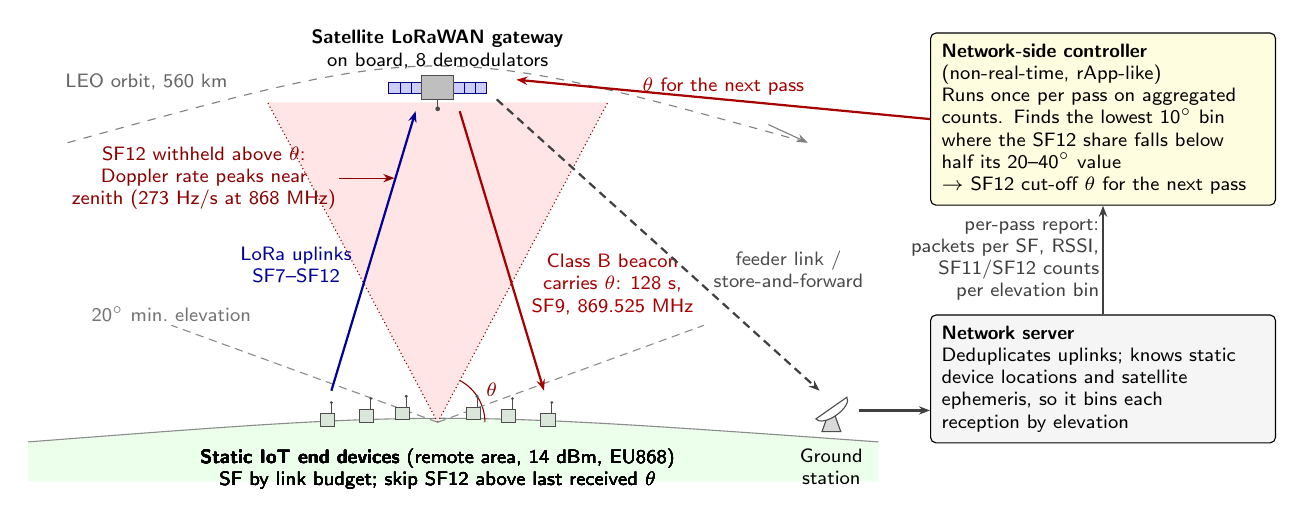
\begin{tikzpicture}[font=\sffamily\scriptsize, >={Stealth[length=4pt]},
  box/.style={draw, rounded corners=2pt, align=left, text width=4.1cm, inner sep=4pt, fill=black!4},
  lbl/.style={align=center, inner sep=1pt},
  up/.style={->, thick, blue!60!black},
  down/.style={->, thick, red!65!black},
  net/.style={->, thick, black!75},
]
% ---------- satellite icon ----------
\newcommand{\sat}[3]{% x, y, opacity
  \begin{scope}[shift={(#1,#2)}, opacity=#3]
    \fill[blue!20, draw=blue!50!black, line width=0.3pt] (-0.62,-0.07) rectangle (-0.2,0.07);
    \fill[blue!20, draw=blue!50!black, line width=0.3pt] (0.2,-0.07) rectangle (0.62,0.07);
    \foreach \u in {-0.48,-0.34,0.34,0.48} \draw[blue!50!black, line width=0.2pt] (\u,-0.07) -- (\u,0.07);
    \fill[black!25, draw=black!70, line width=0.4pt] (-0.2,-0.15) rectangle (0.2,0.15);
    \draw[black!70, line width=0.4pt] (0,-0.15) -- (0,-0.25);
    \fill[black!70] (0,-0.27) circle (0.03);
  \end{scope}}
% ---------- device icon ----------
\newcommand{\dev}[2]{%
  \begin{scope}[shift={(#1,#2)}]
    \fill[green!35!black!15, draw=black!70, line width=0.3pt] (-0.09,0) rectangle (0.09,0.16);
    \draw[black!70, line width=0.3pt] (0.05,0.16) -- (0.05,0.3);
    \fill[black!70] (0.05,0.3) circle (0.02);
  \end{scope}}

% ---------- ground ----------
\fill[green!8] (-0.2,0.35) .. controls (5,0.75) .. (10.6,0.35) -- (10.6,-0.15) -- (-0.2,-0.15) -- cycle;
\draw[black!45] (-0.2,0.35) .. controls (5,0.75) .. (10.6,0.35);

% ---------- orbit ----------
\draw[dashed, black!50] (0.3,4.15) .. controls (5,5.45) .. (9.7,4.15);
\draw[->, black!50] (9.2,4.38) -- (9.7,4.15);
\node[lbl, black!60, anchor=south] at (1.3,4.78) {LEO orbit, 560 km};

% ---------- elevation geometry from the device cluster ----------
\coordinate (A) at (5,0.6);
\fill[red!10] (A) -- ($(A)+(118:4.6)$) -- ($(A)+(62:4.6)$) -- cycle;
\draw[red!55!black, densely dotted] (A) -- ($(A)+(118:4.6)$);
\draw[red!55!black, densely dotted] (A) -- ($(A)+(62:4.6)$);
\draw[red!55!black] ($(A)+(0:0.6)$) arc (0:62:0.6);
\node[red!55!black] at ($(A)+(31:0.8)$) {$\theta$};
\draw[black!45, densely dashed] (A) -- ($(A)+(20:3.6)$);
\draw[black!45, densely dashed] (A) -- ($(A)+(160:3.6)$);
\node[lbl, black!55, anchor=south] at ($(A)+(160:3.6)$) {20$^\circ$ min.\ elevation};
\node[lbl, red!55!black, anchor=east] (cone) at (3.75,3.7) {SF12 withheld above $\theta$:\\Doppler rate peaks near\\zenith (273 Hz/s at 868 MHz)};
\draw[red!55!black, ->, thin] (cone.east) -- (4.45,3.7);

% ---------- satellite ----------
\sat{5}{4.85}{1}
\node[lbl, anchor=south] at (5,5.05) {\textbf{Satellite LoRaWAN gateway}\\on board, 8 demodulators};

% ---------- devices ----------
\foreach \x/\y in {3.6/0.55,4.1/0.6,4.55/0.63,5.45/0.63,5.9/0.6,6.4/0.55} \dev{\x}{\y}
\node[lbl, anchor=north] at (5,0.3) {\textbf{Static IoT end devices} (remote area, 14 dBm, EU868)\\SF by link budget; skip SF12 above last received $\theta$};

% ---------- uplinks and beacon ----------
\draw[up] (3.65,1.0) -- (4.72,4.55);
\node[lbl, blue!60!black, anchor=east] at (3.95,2.6) {LoRa uplinks\\SF7--SF12};
\draw[down] (5.28,4.55) -- (6.35,1.0);
\node[lbl, red!65!black, anchor=west] at (6.15,2.35) {Class B beacon\\carries $\theta$: 128 s,\\SF9, 869.525 MHz};

% ---------- ground station ----------
\begin{scope}[shift={(10.0,0.48)}]
  \draw[black!70, fill=black!15] (-0.12,0) -- (0.12,0) -- (0.04,0.22) -- (-0.04,0.22) -- cycle;
  \draw[black!70, fill=white, rotate around={35:(0,0.3)}] (-0.24,0.3) arc (180:360:0.24 and 0.11) -- cycle;
\end{scope}
\node[lbl, anchor=north] at (10.0,0.3) {Ground\\station};
\draw[net, densely dashed] (5.75,4.7) -- (9.85,1.0) node[pos=0.66, above right, lbl, black!70] {feeder link /\\store-and-forward};

% ---------- network side ----------
\node[box] (ns) at (13.45,1.15) {\textbf{Network server}\\Deduplicates uplinks; knows static\\device locations and satellite\\ephemeris, so it bins each\\reception by elevation};
\node[box, fill=yellow!12] (ctl) at (13.45,4.45) {\textbf{Network-side controller}\\(non-real-time, rApp-like)\\Runs once per pass on aggregated\\counts. Finds the lowest 10$^\circ$ bin\\where the SF12 share falls below\\half its 20--40$^\circ$ value\\$\rightarrow$ SF12 cut-off $\theta$ for the next pass};
\draw[net] (10.35,0.75) -- (ns.west |- 10.35,0.75);
\draw[net] (ns.north) -- (ctl.south) node[midway, left, lbl, align=right, black!75] {per-pass report:\\packets per SF, RSSI,\\SF11/SF12 counts\\per elevation bin};
\draw[down] (ctl.west) -- (6.0,4.95) node[pos=0.5, above, lbl, red!65!black] {$\theta$ for the next pass};
\end{tikzpicture}
\end{document}
